\let\negmedspace\undefined
\let\negthickspace\undefined
\documentclass[journal]{IEEEtran}
\usepackage[a5paper, margin=10mm, onecolumn]{geometry}
%\usepackage{lmodern} % Ensure lmodern is loaded for pdflatex
\usepackage{tfrupee} % Include tfrupee package

\setlength{\headheight}{1cm} % Set the height of the header box
\setlength{\headsep}{0mm}     % Set the distance between the header box and the top of the text

\usepackage{gvv-book}
\usepackage{gvv}
\usepackage{cite}
\usepackage{amsmath,amssymb,amsfonts,amsthm}
\usepackage{algorithmic}
\usepackage{graphicx}
\usepackage{textcomp}
\usepackage{xcolor}
\usepackage{txfonts}
\usepackage{listings}
\usepackage{enumitem}
\usepackage{mathtools}
\usepackage{gensymb}
\usepackage{comment}
\usepackage[breaklinks=true]{hyperref}
\usepackage{tkz-euclide} 
\usepackage{listings}
% \usepackage{gvv}                                        
\def\inputGnumericTable{}                                 
\usepackage[latin1]{inputenc}                                
\usepackage{color}                                            
\usepackage{array}                                            
\usepackage{longtable}                                       
\usepackage{calc}                                             
\usepackage{multirow}                                         
\usepackage{hhline}                                           
\usepackage{ifthen}                                           
\usepackage{lscape}
\begin{document}
\bibliographystyle{IEEEtran}
\title{1.4.17}
\author{EE25BTECH11002 - Achat Parth Kalpesh }
{\let\newpage\relax\maketitle}
\renewcommand{\thefigure}{\theenumi}
\renewcommand{\thetable}{\theenumi}
\setlength{\intextsep}{10pt} % Space between text and floats
\numberwithin{equation}{enumi}
\numberwithin{figure}{enumi}
\renewcommand{\thetable}{\theenumi}
\parindent 0px



Question:\\
Find the coordinates of the points of trisection \brak{\text{i.e. points dividing to three equal parts}} of the line segment joining the points $\vec{A}$ \brak{2,-2} and $\vec{B}$ \brak{-7,4}.\\
\solution\\
Let the given points be represented by the vectors $\vec{A}$ and $\vec{B}$.
\begin{align*}
    \vec{A} = \myvec{2\\-2}, \quad \vec{B} = \myvec{-7\\4}
\end{align*}
The points of trisection, let's call them P and Q, divide the line segment AB into three equal parts.
This means that point P divides AB in the ratio 1:2, and point Q divides AB in the ratio 2:1

The position vector of a point dividing the line segment joining points $\vec{A}$ and $\vec{B}$ in the ratio $m:n$ is given by the section formula:
\begin{align*}
\frac{n \vec{A} + m \vec{B} }{m+n}
\end{align*}
For the first point of trisection, $\vec{P}$ \brak{\text{ratio 1:2 }} \\
Here, $m=1$ and $n=2$.
\begin{align*}
    \vec{P} &= \frac{2 \vec{A} + 1 \vec{B}}{1+2} \\
      &= \frac{1}{3} \brak{ 2\myvec{2\\-2} + 1\myvec{-7\\4}} \\
      &= \frac{1}{3} \brak{\myvec{4\\-4} + \myvec{-7\\4}} \\
      &= \frac{1}{3} \myvec{4-7\\-4+4} \\
      &= \frac{1}{3} \myvec{-3\\0} \\
    \implies \vec{P} &= \myvec{-1\\0}
\end{align*}
So, the coordinates of the first point of trisection are $\vec{P}$ \brak{-1, 0}

For the second point of trisection, $\vec{Q}$ \brak{\text{ratio 2:1 }}

Here, $m=2$ and $n=1$.
\begin{align*}
    \vec{Q} &= \frac{1 \vec{A} + 2 \vec{B}}{2+1} \\
      &= \frac{1}{3} \brak{ 1\myvec{2\\-2} + 2\myvec{-7\\4}} \\
      &= \frac{1}{3} \brak{ \myvec{2\\-2} + \myvec{-14\\8}} \\
      &= \frac{1}{3} \myvec{2-14\\-2+8} \\
      &= \frac{1}{3} \myvec{-12\\6} \\
\implies \vec{Q} &= \myvec{-4\\2} 
\end{align*}

\begin{figure}[h]
    \centering
    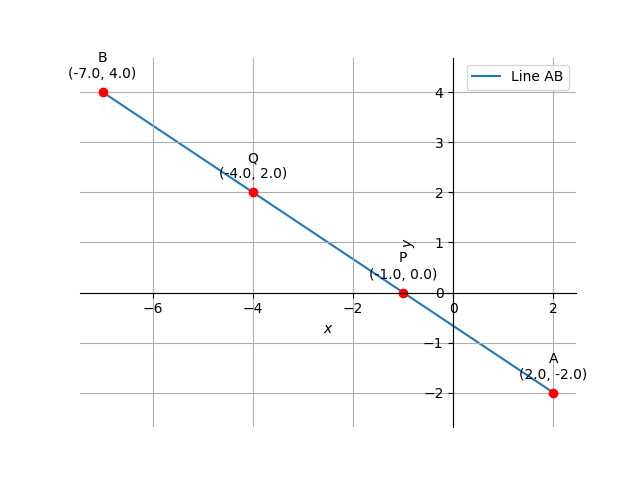
\includegraphics[width=\columnwidth]{figs/Plot_C.png}
    \caption{Graph}
    \label{fig:fig}
 \end{figure}


So, the coordinates of the second point of trisection are $\vec{Q}$ \brak{-4, 2}

Therefore, the coordinates of the points of trisection are \brak{-1, 0} and \brak{-4, 2}
\end{document}